\documentclass[../mattg_ti-fii_lit-review.tex]{subfiles}

\subsection{Primer on TI materials}
In the last two decades there has been a vast discovery of new materials that exhibit phenomenal properties interesting for condensed matter physics research. Usually these materials are stumbled upon experimentally, however in the case of topological materials the setting and expectation was purely theoretical.

Topological insulators (TIs) attract interest because of their unique properties related to electronics. 2D and 3D compounds have edge and surface electronic states respectively, and these states exhibit useful properties such as momentum-spin locking (or localised spin densities) and suppressed back-scattering.

These properties may be used for applications like directing currents that are spinful, ie, exherting magnetic fields or used in spintronics, as well as providing currents that are rhobust with low resistance due to ensured conductivity.

%TODO: Talk about general origins of the field of TIs. Lead into hall effect.

\subsection{History through Hall effects}

\begin{figure}[H]\label{fig:ti_qh-trio}
	\centering
	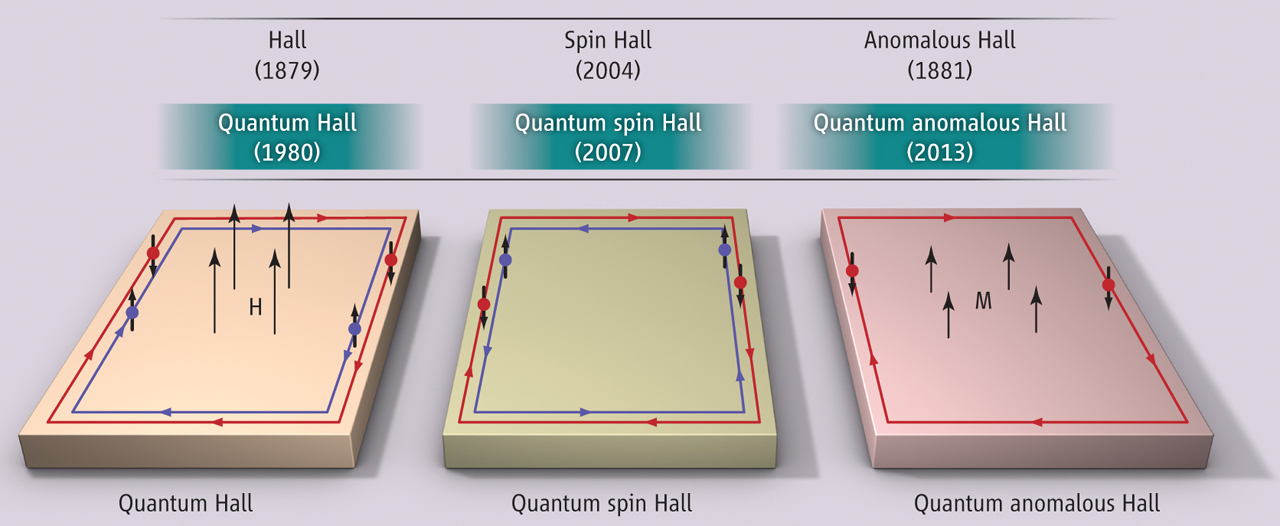
\includegraphics{ti_qh-trio.jpg}
	\caption{The three QH states discovered thus far \cite{oh_complete_2013}}
\end{figure}

\subsubsection{Quantum Hall Effect}\label{sec:QHE}

The quantum hall effect (QHE) was first discovered in MOSFET \footnote{Metal-oxide semiconductor field effect transistors} transistors 1980\cite{klitzing_new_1980}, through a 2 dimensional electron gas (2DEG) found at the interface of a bulk semiconductor and the gate oxide.  %TODO:Cite Klitzing et all 1980.

When introducing a mangetic field to materials, you can produce something called Landau quantisation. You can think of the physical mechanism as the quantisation of cyclotron orbits for charged particles in magnetic fields \footnote{The reason for cyclotron orbits is due to the single valued electron wavefunction, ie $\oint \vec{P}\cdot d\vec{r} = 2\pi N$}. This has the effect of creating new bands called "Landau Levels", that each posess large numbers of orbitals. The degeneracy of the level goes as 

\begin{equation}
	\text{Degeneracy} = \frac{B\times A}{\phi_0}=\frac{B\times A}{h/e}
\end{equation}

This means for some Fermi energy, that you can choose the magnetic field to appropriate values to fill these Landau levels. 

\begin{figure}[H]\label{fig:ti_qhe}
	\centering
	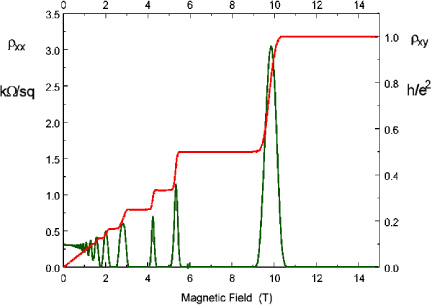
\includegraphics[width=\linewidth/2]{ti_qhe}
	\caption{The quantum Hall effect. \\Courtesy of D.R. Leadley, Warwick University 1997.}
\end{figure}

The QHE looks finely tuned, but because of electrons interacting at the edge there is a confinement of edge states \cite{haldane_topological_2018}.  The edge states dominate transport when the Landau levels of the bulk are filled. Because they are dissapationless, the resistivity $\rho_{xx}$ of the system vanishes, before reaching the next Landau level, where scattering between bulk states can occur again. This is the hallmark\footnote{Although unrelated to the Hall effect, get the pun? Haha.} of topological states, where there exists some states between different phasese of matter.  

The Hall resistivity $\rho_{xy}$ exhibits quantized levels however.

\begin{equation} \label{eqn:qhe-conductivity}
\sigma_{xy}=\nu \frac{e^2}{h}
\end{equation}

Thouless (who later received the noble prize in 2016, before passing away in 2019), Kohmoto, Nightingale, and den Nijs (TKNN) \cite{thouless_quantized_1982} where interested in gapped bulk systems but with conductive edges and a periodic lattice potential. These systems had been argued for explaining the QHE by Laughlin\cite{laughlin_quantized_1981} and the integer effects had earlier been demonstrated theoretically by Hofstadter's Butterfly\cite{hofstadter_energy_1976}. TKNN recognised that \textbf{K} space maps to a non-trivial hilbert space for the QHE; the space has a topology. This topology can be specified by the integer $\nu$ which also corresponds to the hall conductance above in Eq. \ref{eqn:qhe-conductivity}. In particular, their calculations only depended on details of the wavefunctions of the bandstructure. 

What makes this fascinating is that the QHE is a clear example of macroscopic quantum phenomena. Other such phenomena include Bose Einstein Condensation, where many atoms condense into the same uniform quantum state, and superconductivity where the pairing of electrons (Cooper pairs) also produce a new phase of macroscopic quantum behaviour. %TODO check this...


\textcolor{red}{Show calculation of berry phase of the bloch wave function calculated around the BZ boundary divided by 2 pi} %TODO

For the QHE to occur, the Landau quantisation opens gaps in the band structure of the material, and the chemical potential is situated within this gap. In a classical picture, the boundaries of the material cannot sustain these cyclotron orbit, because of the phase transition to an ordinary insulator, rather than the QHE insulator, and so edge channels open in a \textbf{bulk-boundary correspondence}. 

Note that the QHE does not preserve \textbf{time reversal} (TR) \textbf{symmetry}, as charge carriers experience different forces due to the magnetic field when their direction is inverted. The magnetic field breaks TR symmetry. You can see this in the two degrees of freedom in the system; For an out of plane magnetic field, charge is separated into two lanes, and those channels move a particular direction, ie forward above for electrons, backward below for holes. Reversing the direction of carriers yields the same channels but switched, forward above for holes, backward below for electrons. 

\subsubsection{Quantum Spin Hall Effect}\label{sec:QSHE}
The spin hall was observed in 2004 by Kato \etal{} \cite{kato_observation_2004}, where for particular semiconductors a spin density was observed rather than a charge density, like in the regular hall effect.
The origins for such an phenomenon are similar to that of the \hyperref[sec:QAHE]{quantum anomalous Hall effect} in ferromagnets, sometimes being extrinsic, sometimes intrinsic. Intrinsically, the \textbf{Berry curvature} of the electronic valence-band Bloch wave functions result in spin-Hall effect. 

The spin Hall insulator was proposed by Zhang's group\cite{murakami_spin-hall_2004}, where the \textbf{Berry phase} is finite implying a finite spin Hall conductivity. While this idea did not "generate spin currents due to an absense of any electrons at the Fermi level"\cite{ando_topological_2013}, it allowed further exploration to find it quantised version, a quantum spin Hall (QSH) insulator \cite{bernevig_quantum_2006, kane_z_2005,kane_quantum_2005}.

In a real 1D system with spin, you have a regular four degrees of freedom; Spin can move either direction, and can move forward and backward. This could be separated into two copies of the QH system - spin up moving forward with spin down moving backward at the top, and spin down moving forward with spin up moving backward on the bottom. This is referred to the quantum spin Hall effect (QSHE).
But what is the key ingredient that allows this separation of states to occur? In the QHE, it's the magnetic field that breaks time reversal symmetry. For QSH insulators, the essential ingredient is \hyperref[sec:SOC]{spin orbit coupling} (SOC).

An important step made by Kane and Mele\cite{kane_z_2005} was finding a ``topological invariant'' to characterize the QSH insulator states using an index. This index is called the $Z_2$ index. Topological invariants have appeared before. In the \hyperref[sec:QHE]{QHE}, the TKNN invariant $\mu$, where the quantised conductance is proporational to $\nu$. The consequence of the $Z_2$ index is it maps the parity of the number of times the 1D edge state crosses the Fermi level. An odd parity ensures the existance of an edge state and consequently the phase of a topological insulator. The result is significant in it shows how topological phases exist in band structures of insulators, and do not require  external magnetic fields breaking TRS like in the QHE \cite{ando_topological_2013}.

Whilst Kane and Mele used their SOC model to investigate the bandgap opening of graphene, SOC is very difficult to experimentally detect in graphene due to the low coupling strength, compared to that of heavier species. Berneveig et al. \cite{bernevig_quantum_2006}  (Zhang's group) instead proposed a $Z_2$ model for the band structure of mercury telluride (HgTe). They predicted a CdTe/HgTe/CdTe quantum well would give rise to the QSH effect, when the HgTe layer reached a certain critical thickness. Experimental observation was confirmed soon thereafter by K\"onig \cite{konig_quantum_2007}, who observed a quantized conductivity $\sigma_{xx}$ of $2e^2/h$, due to two conducting edges. They also observed the thickness dependence.

\subsubsection{Topological insulators}

By this time theorists (Moore \& Balents \cite{moore_topological_2007}, Fu, Kane and Mele\cite{fu_topological_2007}) had already leapt forward and predicted 3D systems that would exhibit quantum spin hall effects. It was at this point that the term ``topological insulator'' was first coined \cite{moore_topological_2007}. This is distinct to the 2D QSH insulators, but analogous in a 3D version. For these systems there was no longer one invariant to determine the topology of a system, but rather 4 separate invariants, for 16 classes of materials. Generally they could be separated into two groups - strong and weak 3D TIs. 

The first prediction for a 3D TI was by Fu and Kane\cite{fu_topological_2007-2}. They predicted that the surface states of bismuth antimony (\bismuthantimony{}) could be observed by looking at angle resolved photo emission (ARPES, see \ref{sec:ARPES}). The signature for non-trivial topology was in observing surface states crossing the Fermi energy between two TR-invariant momenta \cite{fu_topological_2007-2} %TODO - Understand this last sentence and why ARPES can do this.
This was observed in the same system by Hsieh \etal \cite{hsieh_topological_2008}. 


\subsubsection{Quantum Anomalous Hall Effect}\label{sec:QAHE}
https://science-sciencemag-org.ezproxy.lib.monash.edu.au/content/340/6129/167

``QHE can also occur in some insulators with TRS, broken by current loops, or magnetic ordering, but without Landau levels or external magnetic fields, where it is considered the QAHE. The first Chern number can give the quantized Hall conductance.''
QAHE can occur by the introduction of a ferromagnetic layer.

\subsection{Relevant theory and phenomena}
\subsubsection{Topological field theory}
In 2001 the QHE state was generalized to a 4D TR-invariant state by Zhang and Hu, and was generalized by to field theory by Bernevig \etal{}. It was also shown later by Zhang how the $Z_2$ topology could be described in this field theory, and be reduced to the 2D and 3D cases.

Pratically according to Ando's review \cite{ando_topological_2013}, this is useful for descibing electromagnetic responsese of TIs and predicting magnetoelectric effects.

\subsubsection{Dirac Fermions}
Within graphene, mentioned earlier for the Kane and Mele SOC model \cite{kane_quantum_2005}, the 2D electron gas over the carbon honeycomb lattice creates interesting band structure features called ``Dirac cones". 
Generally in semiconductors and other insulators, the electronic bands eitherside of the bandgap become quite flat with curvature in momentum space.

\subsection{Topological Invariants}

\subsection{Symmetries}
\subsubsection{Inversion Symmetry}
Bulk states are spin-degenerate, because of combination of space-inversion symmetry ($E(k,\uparrow) = E(-k, \uparrow)$) and time-reversal symmetry ($E(k,\uparrow) = E(-k, \downarrow)$) \cite{hsieh_observation_2009}.
At the surface however where inversion symmetry is broken, spin-orbit interaction can lift the spin degeneracy. 

\subsubsection{Kramers Theorem}
Kramers theorem requires particular points mapped from the BZ (Brouillin zone) to retain spin degeneracy. For \bismuthantimony{}, spin states split at the surface by spin-orbit interaction must remain spin-degenerate at four special TR invariant momenta; $\Gamma$, and three equivalent $M$ points. Ref in Hsieh \etal{}\cite{hsieh_observation_2009}. %TODO fixup quote original reference.

\subsection{Spin-Orbit Coupling}\label{sec:SOC}
Spin-orbit coupling (SOC) is coupling of both spin and orbital angular momentum properties of particles. Spin provides a magnetic moment, and the motion of the charged electron through its orbital angular momentum also provides a magnetic moment. From the electrons point of view, it can be considered to be the interaction of the electron's spin with the orbital motion of the nucleus.

This coupling causes splitting, similar to Zeeman splitting, of electronic energy levels. For different atoms, the SOC is different, with the trend that heavier atoms have a larger SOC \cite{herman_relativistic_1963}. 

This type of coupling doesn't break time-reversal symmetry like magentic field for QHE, but can lead to the \hyperref[sec:QSHE]{QSHE}, where electrons differentiated by their spin move in opposite directions.

\subsubsection{Rashba Effect}

\subsubsection{Dresselhaus Effect}


\subsection{Berry Phase}
\cite{berry_quantal_nodate}
\cite{simon_holonomy_1983}

\subsection{Kubo formula}


\subsection{Band inversion}

\subsection{2D Dirac Systems}

\subsection{Materials \& Growths}
\subsubsection{\bismuthselinide{}}

\subsubsection{\bismuthtelluride{}}

\subsubsection{}
